\documentclass[a4paper,10pt,ngerman]{scrartcl}
\usepackage{babel}
\usepackage[T1]{fontenc}
\usepackage[utf8x]{inputenc}
\usepackage[a4paper,margin=2.5cm,footskip=0.5cm]{geometry}

% Die nächsten drei Felder bitte anpassen:
\newcommand{\Aufgabe}{Aufgabe 3: Hex-Max} % Aufgabennummer und Aufgabennamen angeben
\newcommand{\TeilnahmeId}{63175}                  % Teilnahme-ID angeben
\newcommand{\Name}{Lars Noack}             % Name des Bearbeiter / der Bearbeiterin dieser Aufgabe angeben


% Kopf- und Fußzeilen
\usepackage{scrlayer-scrpage, lastpage}
\setkomafont{pageheadfoot}{\large\textrm}
\lohead{\Aufgabe}
\rohead{Teilnahme-ID: \TeilnahmeId}
\cfoot*{\thepage{}/\pageref{LastPage}}

% Position des Titels
\usepackage{titling}
\setlength{\droptitle}{-1.0cm}

% Für mathematische Befehle und Symbole
\usepackage{amsmath}
\usepackage{amssymb}

% Für Bilder
\usepackage{graphicx}

% Für Algorithmen
\usepackage{algpseudocode}

% Für Quelltext
\usepackage{listings}
\usepackage{color}
\definecolor{mygreen}{rgb}{0,0.6,0}
\definecolor{mygray}{rgb}{0.5,0.5,0.5}
\definecolor{mymauve}{rgb}{0.58,0,0.82}
\lstset{
  keywordstyle=\color{blue},commentstyle=\color{mygreen},
  stringstyle=\color{mymauve},rulecolor=\color{black},
  basicstyle=\footnotesize\ttfamily,numberstyle=\tiny\color{mygray},
  captionpos=b, % sets the caption-position to bottom
  keepspaces=true, % keeps spaces in text
  numbers=left, numbersep=5pt, showspaces=false,showstringspaces=true,
  showtabs=false, stepnumber=2, tabsize=2, title=\lstname
}
\lstdefinelanguage{JavaScript}{ % JavaScript ist als einzige Sprache noch nicht vordefiniert
  keywords={break, case, catch, continue, debugger, default, delete, do, else, finally, for, function, if, in, instanceof, new, return, switch, this, throw, try, typeof, var, void, while, with},
  morecomment=[l]{//},
  morecomment=[s]{/*}{*/},
  morestring=[b]',
  morestring=[b]",
  sensitive=true
}

% Diese beiden Pakete müssen zuletzt geladen werden
\usepackage{hyperref} % Anklickbare Links im Dokument
\usepackage{cleveref}

% Daten für die Titelseite
\title{\textbf{\Huge\Aufgabe}}
\author{\LARGE Teilnahme-ID: \LARGE \TeilnahmeId \\\\
	    \LARGE Bearbeiter/-in dieser Aufgabe: \\ 
	    \LARGE \Name\\\\}
\date{\LARGE\today}

\begin{document}

\maketitle

\setcounter{tocdepth}{3}
\tableofcontents

\vspace{0.5cm}

\section{Lösungsidee}

Da ich sehr viel Zeit für die Bohnusaufgabe verwendet habe, für die mir die Zeit aufgrund von der Schule ausgieng, ist diese Lößung pottentiell nicht ganz ausgereift.

\subsection{Vereinfachungen und Regeln}

Um meine Lößung zu verstehen ist es wichtig zuerst ein paar Regeln zu etablieren, die Beschreiben wann eine potentielle Lößung richtig sein kann. Da dies einfacher mit Streichhölzern wie mit Sieben-Segment-Anzeigen ist, gehen wir gedanklich davon aus und etablieren die Regel, dass sich die Länge der gegebenen Zahl nicht ändern darf. Dies ist der Fall, da man nicht einfach neue Anzeigen kaufen kann um die Zahl länger zu machen, und nicht einfach Anzeigen nicht nutzen kann, da die Zahl dann kleiner werden würde als ohne überhaupt einen Zug zu machen.

Jetzt ist es wichtig zu beschreiben, was überhaupt ein Zug ist. Ein Zug ist das verschieben eines Streichholzes. Man kann dies aber auch so formulieren, dass man ein Streichholz weglegt, und es wieder hin legt. Dies klingt wie das gleiche, was es aber nicht ist. Definiert ist nämlich nur dass man das Streichholz wieder zurücklegt, und nicht wann. Das heißt man kann eine Ziffer zu einer anderen umwandeln in dem man 2 Streichhölzer wegnimmt. Dann kann man einfach zu anderen Ziffern gehen und diese auch nach belieben umwandeln. Am Ende muss man nur so viele Weggenommen haben, wie man auch Welche hingelegt hat.

Die Anzahl der Weggenommenen Streichhölzer kürze ich zur vereinfachung mit $R$\footnote{number of removed matches} ab, die Anzahl der Hinzugefügten mit $A$\footnote{number of addet matches}. $m$ ist die Maximalzahl an Umlegungen bzw. an Zügen und $z$ ist die Zahl an tatsächlich gebrauchten Zügen.

Wenn man schauen will ob ein Ergebniss überhaupt mit beliebigen Umlegungen erreicht werden kann vergleicht man $A$ und $R$. Wenn beide gleich sind, kann das Ergebniss erreicht werden, sonst nicht. Will man die Anzahl an tatsächlich verbrauchten Zügen wissen gilt $z = R = A$. Ist $z > m$ kann dieses Ergebniss auch nicht erreicht werden, da zu wenig Züge vorhanden sind.

\paragraph{Zusammengefasst gilt}

\begin{enumerate}
  \item Die Zahl an 'Streichhölzer' die weggenommen wurde ist $R$.
  \item Die Zahl an 'Streichhölzer' die hinzugefügt wurden ist $A$.
  \item Die Anzahl an Zügen $z$ ist $z = max(A, R)$.
  \item Wenn $A \neq R$ dann ist die Lösung nich möglich.
  \item Wenn $z > m$ dann ist die Lösung auch nicht möglich.
\end{enumerate}

\subsection{Das finden der Einzelnen Umlegungen}

In der Aufgabenstellung steht dies: 'Das Programm soll nach jeder Umlegung den Zwischenstand, also die aktuelle Belegung
der Positionen ausgeben'. Ich bekomme aber lediglich die größte\footnote{vermutlich größte} Zahl ohne die Zwischenschritte, was dem geschuldet ist dass ich die 'Streichhölzer' zwischenspeichere und nutze wenn ich will. Die Zwischenschritte zu berechnen ist aber vergleichsweise einfach machbar. Man vergleicht jedes Segment bei jeweils der Startzahl und dem Ergebnis. Wenn dieses Segment verändert wurde merkt man sich das Segment und ob das Segment an oder aus gemacht wurde. Dann schaut man weiter bis man ein Segment gefunden hat, bei dem es statt an, aus gemacht wurde oder anders herum. Dann kann man von der Startzahl die Erste Umlegung bei diesen beiden Segmenten machen. Dies macht man so oft lang, bis man bei dem Ergebniss angekommen ist\footnote{man sollte diese Zwischenergebnisse natürlich auch ausgeben}.

\subsection{Die größte Zahl mit unendlich Umlegungen}  

Wenn ich die größtmögliche Zahl mit unendlichen Umlegungen finde, muss ich diese weniger verändern. Bei dem 5. Beispiel muss ich z.B statt von 0 auf 1369 Züge von 1425 auf 1369 Züge kommen. Dies ist einfacher. Aber wie bekomme ich die größstmögliche Zahl. Um es kurz zu fassen zähle ich die Segmente die bei der gegebenen Zahlenkombination an sind. Dann setzte ich von der vordersten Stelle zur hintersten auf die größtmöglichte Zahl. Ausgeschlossen sind alle Zahlen die es verhindern würden, dass die vorhin gezählte Anzahl an Segmenten an ist. Man kann nämlich pro Ziffer höchstens 7 Segmente an machen\footnote{8}. Pro Ziffer muss man aber auch mindestens 2 Segmente an machen\footnote{1}.

\subsection{Die Zahl verringern bis es passt}

Das anpassen der größten Zahl mit unendlich Umlegungen mach ich iterativ. Hier beschreibe ich eine iteration, die ich dann wiederhole bis ich nicht mehr zu viele Umlegungen mache.

Ich gehe hier von der kleinsten Stelle zur größten Stelle, da ich den Wert der Zahl so wenig wie möglich verändern will. Bei jeder Ziffer gehe ich dann jede mögliche neue Ziffer durch $i$. Also alle Zahlen ab 15 bis 0. $i$ ist die Zahl in die ich die Ziffer ändern könnte. Bei jedem neuen $i$ schaue ich dann, ob sich die Umlegungen verringern würde, und ob sich die Tendenz zu $A$ oder $R$ sich nicht verstärkt\footnote{Die Tendenz kann durch den iterativen Prozess entstehen}. Ist dies der Fall, dan setze ich die Ziffer auf $i$ und beende diese eine Iteration. Wenn die nicht der fall ist, dann gehe zum nächsten $i$ oder ggf. zur nächsten Ziffer.

\subsection{Mit den übrigen Zügen die Zahl wenn möglich erhöhen}

Das iterative herangehen von oben hat das Problem, dass die Züge meist nicht voll ausgeschöpft werden. Dies ist zwar explitzit laut der Aufgabenstellung erlaubt, jedoch gibt es oft Situationen, bei denen man mit der Ausschöpfung aller Züge noch das Ergebnis erhöhen kann. Um das auszuschliesen nutze ich brute force.

Simples Konzept. Ich schaue bei jeder Ziffer, bei den großen startend, ob ich diese erhöhen kann, speicher die Differenz zwischen $A$ und $R$.
Dann geh ich zu anderen ziffern und schaue ob ich diese erhöhen kann, so dass dieselbe Differnz * -1 einer der gespeicherten Differenzen entspricht. Wenn ändere ich dies.
 
\paragraph{Somit habe ich die Lößung.}

\section{Umsetzung}

\subsection{Generelles}

Um $R$ und $A$ überhaupt bekommen zu können, muss ich zuerst die anordnungen für alle 16 ziffern speichern. Dies mach ich in einem bool-array der länge 7. True heißt, das Segment ist an, False heißt es ist aus. Dieses bool-array speicher ich in einer weiteren liste der Länge 16.

Es gibt $15^2 = 225$ Möglichkeiten den Wert einer Ziffer in einen anderen umzuwandeln. Da ich häufig $R$ und $A$ brauche, welches aus dieser Situation entsteht speicher ich das in einer zweideminsionalen Liste ab. Dann kann ich diese werte so bekommen: $changeHex[from][to][add/remove]$

\subsection{R und A einer Zahl}

Hier geht es nicht um eine Ziffer wie $0xF$ sondern um eine ganze Zahl wie $0xEE4$. $R$ und $A$ dort rauszufinden ist sehr einfach. Ich gehe mi einem for loop über jede ziffer und summiere $A$ und $R$ aus $changeHex$ aufeinander.

\subsection{größte Zahl ohne Zuglimit}

Hier wird es erst interessant. Als erstes brauch ich die maximale Anzahl $maxSeg$ und die minnimale Anzahl $minSeg$ an Segmenten die an sind pro Ziffer. Dies wäre $2$ und $7$. Dann brauch ich auch noch die Anzahl an Segmenten die an sind in der gesammten gegebenen Zahl. Dies nenne ich $leftovers$\footnote{wird gleich klar warum}. Dann initialisiere ich eine leere Liste $hex$ die die neue Zahl speichern wird. Dann starte ich ein for loop der die länge der ursprünglichen hex zahl $n$ läuft. Die Anzahl an noch zu füllenden ziffern ist $i$. Wenn eine Zahl gefunden worde, die funktioniert, wird diese zu $hex$ hinzugefügt und von leftovers wird die Anzahl an Segmenten der neuen Zahl abgezogen. Um die Zahl zu finden wird bei 15 gestartet und runtegezählt bis eine Zahl valid ist. Eine Zahl ist valid, wenn $minSeg \leq leftovers : i \leq maxSeg$.

\begin{algorithmic}[1]
\State hex = []
\State leftovers = givenSegmentAmmount
\For{$leftoverDigits = givenHexLen, \dots, 0$}
\For{$i = 15, \dots, 0$}
\State SegmentsPerDigit = (leftovers - Segments[i]) / leftoverDigits
\If{$minSeg \leq SegmentsPerDigit \leq maxSeg$}
\State hex.append(i)
\EndIf
\EndFor
\EndFor
\end{algorithmic}

\subsection{Die Zahl verringern bis es passt}

Die in Lösungsidee erwähnte Schleife Realisiere ich mit einer while Schleife mit oben genannten bedingungen. Dann iteriere ich mit einem for loop über die Zahl und breche aus dem loop wenn ich etwas geändert habe. Dann schaue ich mit einer for schleife alle möglichen änderungen an, und ob ich die Änderung nehmen sollte, wenn nicht rufe ich continue auf.

Dies mach ich zuerst daran fest, ob die neue tendenz die alte mehr in eine Richtung drückt\footnote{Zeile 7 - 11}. Wenn ja dann kann ich dies nicht nehmen. Dannach mus nur die änderung weniger Züge brauchen als die alte, dann nehme ich diese.


\begin{algorithmic}[1]
\While{currentNeededMoves > maxMoves || adds != removes}
\For{$i = lenHex \dots 0$}
\State changed = False
\State prevTendence = adds - removes

\For{$toDigit = 15 \dots 0$}
\State newTendence = newAdds - newRemoves
\If{tendence < 0 and newTendence < tendence}
\State continue
\ElsIf{tendence > 0 and newTendence > tendence}
\State continue
\EndIf

\If{oldMoves > newMoves}
\State hex[i] = toDigit
\State changed = True
\State break
\EndIf

\EndFor

\If{changed}
\State break
\EndIf
\EndFor

\EndWhile
\end{algorithmic}

\subsection{Die übrigen Züge nutzen}

Nochmal eine kleine Zusammenfassung was ich will. Ich will die Zahl mit meinen übrigen Umlegungen möglichst stark vergrößen. Deshalb fang ich bei den vorderen Stellen an und arbeite mich nach hinten vor, bis keine Züge mehr übrig sind, oder alle Ziffern angeschaut worden sind.

Bei jeder iteration erstelle ich ein dictionary/hash list in dem die Tendenz von jeder Änderung gespeichert wird. 

Wenn alles gespeichert gehe ich mit einem ähnlichen for loop, wie der aller erste ab der jetzigen Stelle jede weitere Stelle durch. Dann lass ich so ein for loop wie bei dem auffüllen des dictionarys laufen, bis ich eine änderung gefunden habe, die die Tendenz hat wie -1 * eine aus dem dictionary. Finde ich keine geh ich zur nächsten Stelle.

\begin{algorithmic}[1]
\For{$i = 0 \dots lenHex$}
\State digit1 = hex[i]

\State possibleChange = $\{\}$

\For{$possibility = 15 \dots digit1 + 1$}
\State possibilityTendence = possibilityAdd - possibilityRemove
\If{possibilityTendence not in possibleChange}
\State possibleChange[possibilityTendence] = posibility
\EndIf 
\Comment{Da ich von groß nach klein Zähle, sind in possibleChange immer die größten Werte}
\EndFor


\For{$j = i+1 \dots lenHex$}
\State foundChange = False

\For{$possibility = 15 \dots 0$}
\State possibilityTendence = possibilityAdd - possibilityRemove
\If{possibilityTendence * -1 in possibleChange}
\State foundChange = True
\State hex[i] = possibleChange[possibilityTendence * -1]
\State hex[j] = possibility
\State break
\EndIf
\EndFor

\If{foundChange}
\State break
\EndIf
\EndFor

\If{noMovesLeft}
\State break
\EndIf
\EndFor

\end{algorithmic}



\section{Laufzeitanalyse}

$n$ ist die Länge der Zahl.

\subsection{größte Zahl ohne Zuglimit}

Diese komplexität ist linear. $O(n)$. Der Grund dafür ist, dass der äußere loop $n$ mal lauft und in dem loop meist 1 mal oder manchmal mehr als 1 mal. Das mehr als 1 mal ist aber unabhängig von $n$

\subsection{Die Zahl verringern bis es passt}

Die theorethische Laufzeitanalyse hierfür ist schwer und sinnlos. Erstens ist das nicht von $n$ abhängig sondern eher von $m$. Dies aber auch nicht, da es eigentlich von $zuegeBeiOhneZuglimit - m \leq 0$ abhängig ist und auf diese Art wird es immer komplexer. Es ist aber meines erachtens nicht wichtig, da es zwar sehr nah ans Ziel herankommt, aber erst der nächste Schritt, der in jedem Beispiel länger braucht, das Ziel erreicht wird.

\subsection{Die übrigen Züge nutzen}

Diese Laufzeit sieht ganz anders aus natürlich gibt es dort immer noch das zufallselement, wie bei den anderen, aber hier spielt das nur eine kleine Rolle, die vernachlässigbar ist.

Die äuserste Schleife läuft $n$ mal wobei $n$ hier wieder die Länge der Zahl ist. In dieser läuft eine Schleife 16 mal was eine Komplexität von $O(16n)$ was gleichzusetzen mit $O(n)$ ist. In der äußeren Schleife ist noch eine schleife die n-i läuft. i ist hierbei die jeweilige Iteration. 
Wenn man dass von vorhin mit dem Kombiniert und die Formel für die Summe aller Integer \footnote{\url{https://researchmaniacs.com/Calculator/SumOfIntegers/Sum-of-integers-from-1-to-100.html}} hinzuzieht kommt man auf $n^2 - n(n+1)/2$. Dies kann als $\frac{n^2 - n}{2}$. Wir können sowol das $-n$ als auch das $/2$ vernachlässigen, was am Ende die Laufzeit $O(n^2)$ ergibt.

\subsection{praktische Laufzeit}

In der untersuchung vernachlässige ich das berechnen der zwischenzüge, da dies erstens vernachlässigbar ist. Zweitens da dieser code eingewoben mit dem rendering code ist, welcher schlecht ist und alles langsamer machen kann. Dies ist also schwehr zu separieren.
\\
\\
Für die praktische Laufzeitanalyse habe ich für jedes n von 10 bis 1000 in 50er Schritten jeweils 100 Aufgaben generiert und die Zeit gemessen. Daraufhin habe ich für jede 100 Aufgaben den Durchschnit und die Standartabweichung berechnet. Diese habe ich geplottet, und eine quadratische Funktion an die Werte angepasst. Wie man sehen kann passt diese zimlich gut, was meine Theoretische Laufzeitanalyse von $O(n^2)$ stützt.
\\
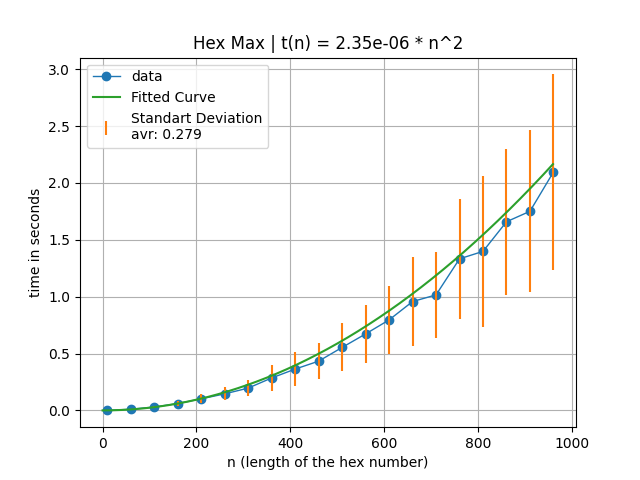
\includegraphics[width=\textwidth]{Laufzeit.png} 

\section{Beispiele}

Ersteinmal vorab, ich habe alle Beispiele gemacht. Um aber alle Zwischenschritte darzustellen, muss ich Bilder rendern, da nicht alle Möglichkeiten einer Sieben-Segment Anzeige einer Zahl entsprechen. Einige Bilder sind jedoch viel zu groß für eine PDF. Diese sind in dem Unterordner 'Solutions' zu finden. Um die Bilder zu öffnen empfehle ich XnView. Alternativ habe ich jeden Schritt, der als Zahl dargestellt werden kann als Zahl im Hexadezimalsystem dargestelt.
\\
\\
$m$: die maximale Anzahl an umlegungen
\\
$n$: die länge der Hex Zahl

\subsection{Winzig}

$m=3$
\\
$n=3$
\\
Startzahl: 0xD24
\\
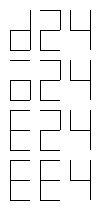
\includegraphics[scale=.5]{solutions/hexmax0.png}

\subsection{Immer noch klein}

$m=8$
\\
$n=10$
\\
\\
Startzahl: 0x509C431B55
\\
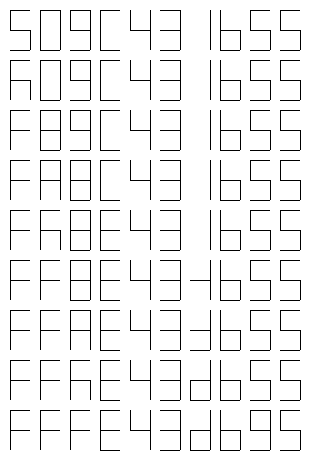
\includegraphics[scale=.5]{solutions/hexmax1.png}

\subsection{nicht groß}

Das Bild ist auf der nächsten Seite, da es eine ganze Seite verbraucht. Die nächsten werden nur als text bzw. als screenshot von Text zu sehen sein. Screenshot von Text wegen den wrapping Limitationen von \TeX.
\\
\\
$m=37$
\\
$n=40$
\\
\\
Startzahl: 0x632b29b38f11849015a3bcaee2cda0bd496919f8
\newpage
\noindent 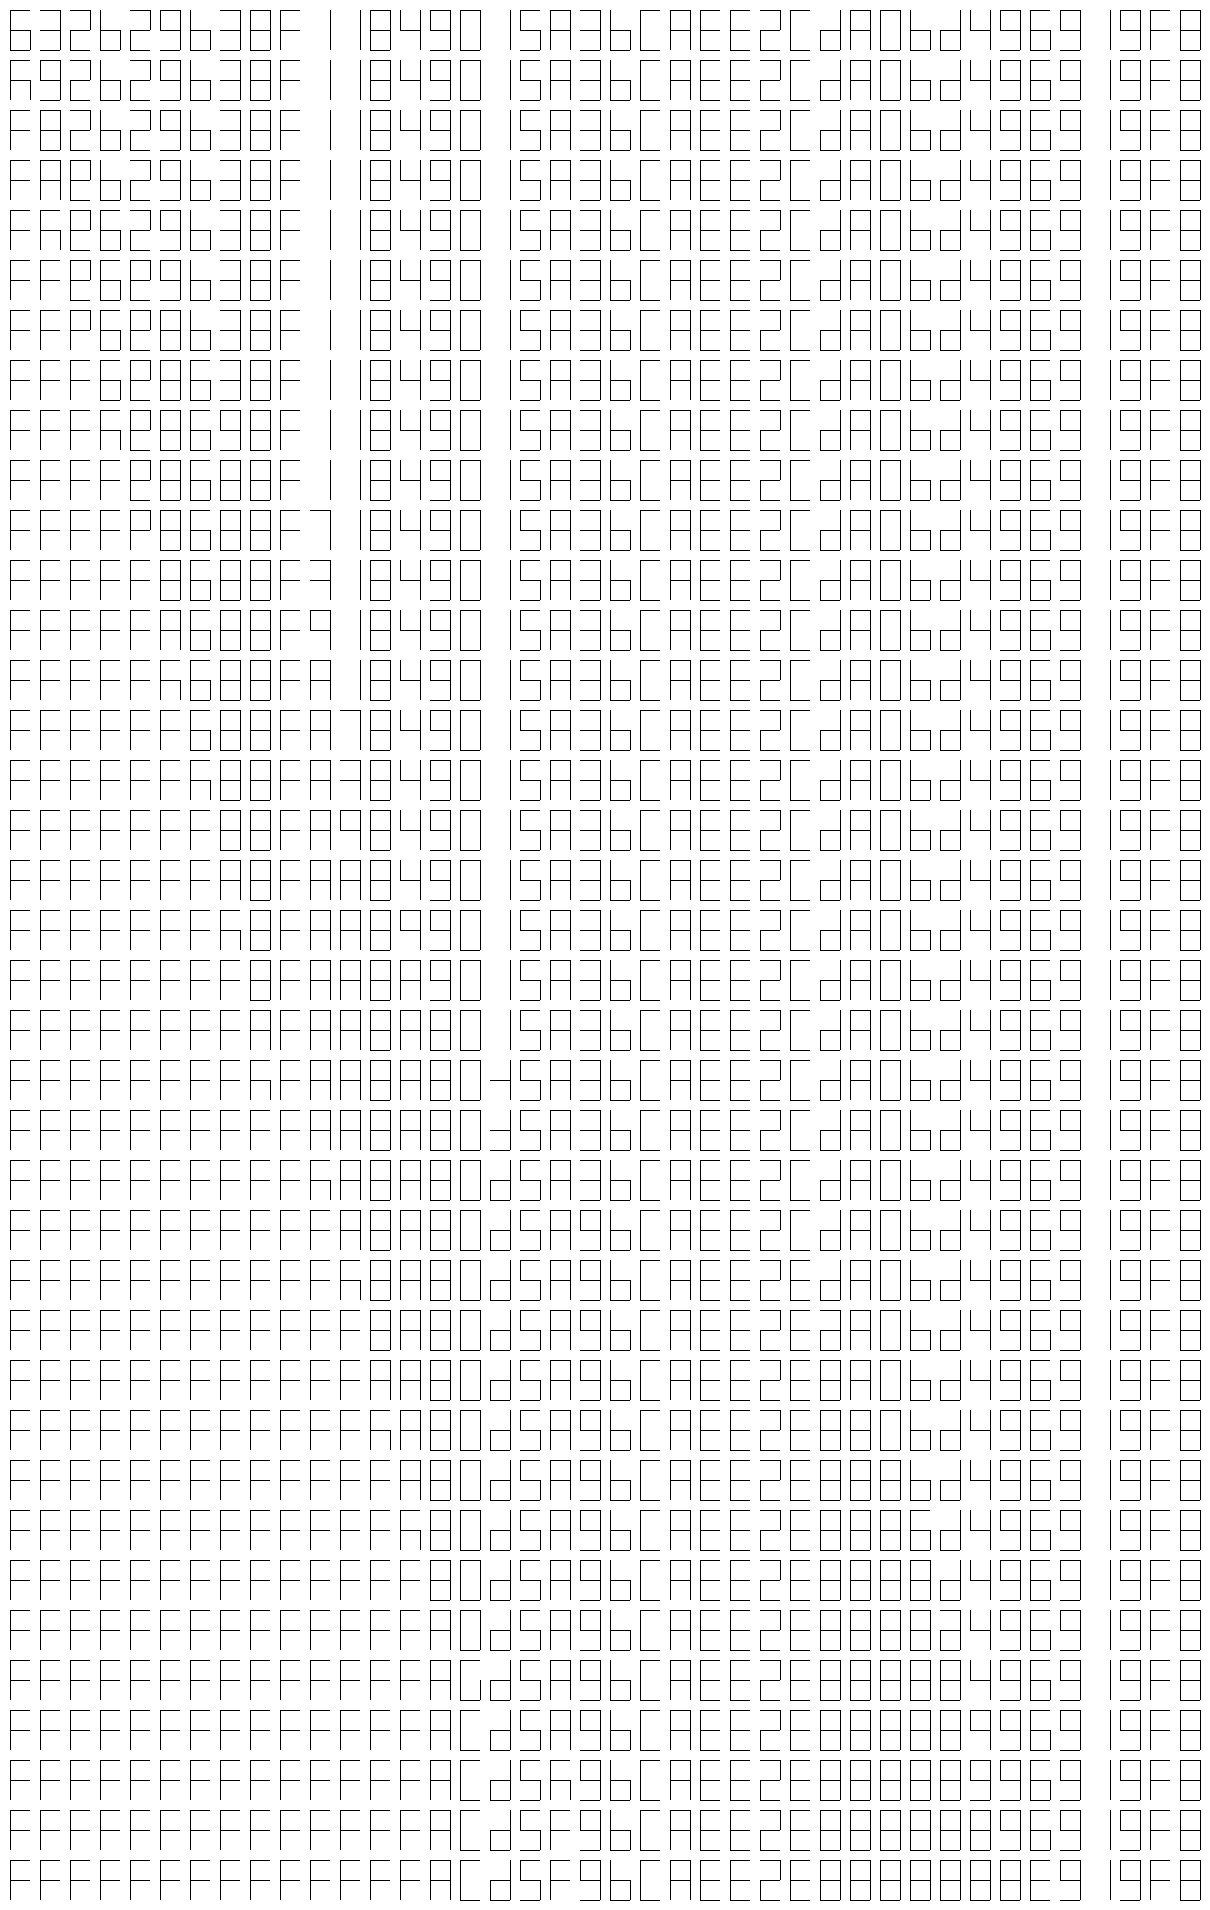
\includegraphics[scale=.4]{solutions/hexmax2.png} 

\subsection{ein bischen groß}

$m=121$
\\
$n=100$
\\
\\
Startzahl: 
\\
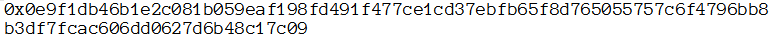
\includegraphics[width=\textwidth]{solutions/startzahl3.png} 
\\
größte Zahl:
\\
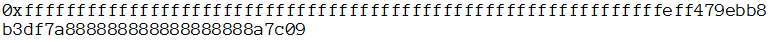
\includegraphics[width=\textwidth]{solutions/endzahl3.png} 

\subsection{immer noch groß}

$m=87$
\\
$n=100$
\\
\\
Startzahl: 
\\
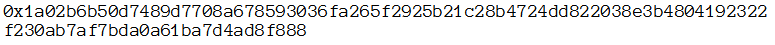
\includegraphics[width=\textwidth]{solutions/startzahl4.png} 
\\
größte Zahl:
\\
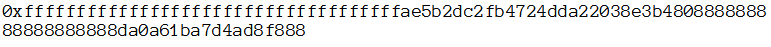
\includegraphics[width=\textwidth]{solutions/endzahl4.png} 

\subsection{O.o}

$m=1369$
\\
$n=1000$
\\
\\
Startzahl: 
\\
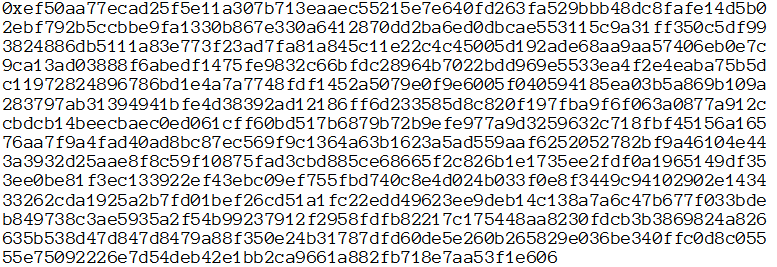
\includegraphics[width=\textwidth]{solutions/startzahl5.png} 
\\
größte Zahl:
\\
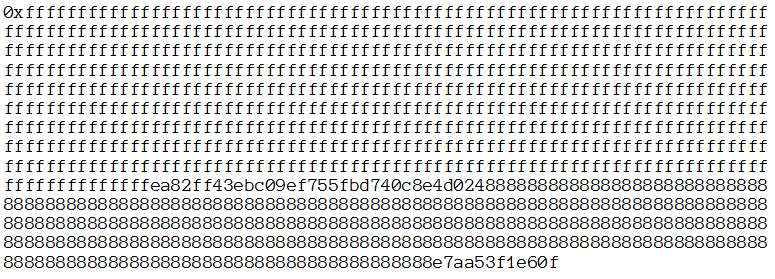
\includegraphics[width=\textwidth]{solutions/endzahl5.png} 




\section{Quellcode}

Der erste Teil des Codes geht klar.

\lstset{
	language=python, 				% Setzt die Sprache
}
\begin{lstlisting}
import json
import numpy as np
import logging
import enum

logging.basicConfig(level=logging.DEBUG, format='%(asctime)s - %(levelname)s - %(message)s')

class Hex(enum.Enum):
    add = "add"
    remove = "remove"
    moves = "moves"
    change = "change"

# read hex.json and store as hex matrix
"""
hex matrix: list of all states of the seven segment display for every hex number
hex sticks: a dictionary with the key being the value of the hex number and the value the number of sticks
"""
with open('hex.json') as f:
    hex_matrix = json.load(f)
    hex_sticks = {}

    # count sticks and save as in dictionary
    for i, number in enumerate(hex_matrix):
        hex_sticks[i] = np.sum(number)
    hex_sticks = dict(sorted(hex_sticks.items(), key=lambda x: x[1]))


# fill up change hex
# liste wie viele striche man von jeder zu jeder zahl hinzufuegen bzw. wegnehmen muss.
change_hex = {}
for hex_1, hex_matrix_1 in enumerate(hex_matrix):
    change_hex[hex_1] = {}

    for hex_2, hex_matrix_2 in enumerate(hex_matrix):
        remove = 0
        add = 0
        for bool1, bool2 in zip(hex_matrix_1, hex_matrix_2):
            if bool1 and not bool2:
                remove += 1
            elif not bool1 and bool2:
                add += 1

        change_hex[hex_1][hex_2] = {Hex.add: add, Hex.remove: remove, Hex.moves: max(add, remove), Hex.change: add - remove}


def print_hex_list(hex_list: list):
    print(''.join([f"{digit:x}" for digit in hex_list]))

def get_sticks(hex_str: str):
    sticks = 0
    for digit in hex_str:
        sticks += hex_sticks[int(digit, 16)]
    return sticks


def get_biggest_hex_infinite(sticks: int, hex_length: int):
    # get biggest hex number with infinite moves
    leftovers = sticks

    min_sticks = hex_sticks[list(hex_sticks)[0]]
    max_sticks = hex_sticks[list(hex_sticks)[-1]]

    # list with integers for each digit
    hex_number = []
    for i in range(hex_length):
        leftover_digits = hex_length - i - 1

        for j in reversed(range(16)):
            possible_leftovers = leftovers - hex_sticks[j]

            if possible_leftovers == 0 and leftover_digits == 0:
                hex_number.append(j)
                break

            if leftover_digits == 0:
                continue

            if possible_leftovers < 0:
                continue
            sticks_per_digit = possible_leftovers / leftover_digits

            if sticks_per_digit < min_sticks:
                continue
            if sticks_per_digit > max_sticks:
                continue

            leftovers = possible_leftovers
            hex_number.append(j)
            break

    if len(hex_number) != hex_length:
        raise Exception('Numbers dont match while generating the biggest hex number with infinite moves')

    return hex_number

def needed_value_between_hex(hex_from: list, hex_to: list) -> (int, int):
    # get needed moves between two hex numbers
    total_added = 0
    total_removed = 0

    for from_digit, to_digit in zip(hex_from, hex_to):
        total_added += change_hex[from_digit][to_digit][Hex.add]
        total_removed += change_hex[from_digit][to_digit][Hex.remove]

    return total_added, total_removed

def needed_moves_between_hex(hex_from: list, hex_to: list) -> int:
    # get needed moves between two hex numbers
    total_added, total_removed = needed_value_between_hex(hex_from, hex_to)

    if total_added != total_removed:
        logging.warning(f"{total_added} != {total_removed}")
        logging.warning(f"{hex_1} -> {hex_2}")

    return max(total_added, total_removed)

def revert_illegal_moves(hex_from: list, hex_to_: list, max_moves: int) -> list:
    if len(hex_from) <= 0 or len(hex_to_) <= 0:
        raise Exception('hex_from or hex_to is empty. Thus the problem is not in revert_illegal_moves')

    hex_to = hex_to_.copy()

    timeout = 500
    iteration = 0
    # the needed_moves in the while loop is performant enough running in about 5 seconds for 5000 iterations
    needed_moves = max_moves+1
    needed_change = 0
    while needed_moves-max_moves > 0 or needed_change != 0:
        iteration += 1
        if iteration > timeout:
            logging.warning('Timeout while reverting moves')
            return hex_to


        needed_adds, needed_removes = needed_value_between_hex(hex_from, hex_to)
        # print(needed_adds, needed_removes)
        needed_moves = max(needed_adds, needed_removes)
        needed_change = needed_adds - needed_removes

        if not (needed_moves-max_moves > 0 or needed_change != 0):
            break

        # print_hex_list(hex_to)
        # print(f"{needed_adds} - {needed_removes} = {needed_change} -> {needed_moves}")

        for i, from_digit in reversed(list(enumerate(hex_to))):
            if hex_from[i] == from_digit:
                continue

            initial_adds = change_hex[hex_from[i]][from_digit][Hex.add]
            initial_removes = change_hex[hex_from[i]][from_digit][Hex.remove]
            initial_moves = max(initial_adds, initial_removes)

            # die adds und removes die in dieser iteration nicht geaendert werden koennen
            # also von inf change ohne diese iteration
            bare_adds = needed_adds - initial_adds
            bare_removes = needed_removes - initial_removes

            # print(f"{i} {from_digit} move {needed_moves} change {needed_change} specific a{adds} r{removes} m{moves} c{changes}")
            new_digit = -1
            for to_digit in reversed(range(16)):
                iter_adds = bare_adds + change_hex[hex_from[i]][to_digit][Hex.add]
                iter_removes = bare_removes + change_hex[hex_from[i]][to_digit][Hex.remove]

                iter_change = iter_adds - iter_removes
                iter_moves = max(iter_adds, iter_removes)

                # print(f"iter {i} {to_digit} add {iter_adds} remove {iter_removes} move {iter_moves} change {iter_change}")

                if needed_change > 0 and iter_change > needed_change:   continue
                if needed_change < 0 and iter_change < needed_change:   continue

                # print("heh", iter_adds, iter_removes)
                if iter_moves < needed_moves:
                    # print("???????????????")
                    new_digit = to_digit
                    break

            if new_digit != -1:
                break


        if new_digit == -1:
            pass
            # print_hex_list(hex_to)
            # logging.warning('No digit found to revert illegal moves (if it occurs only once, it is not an error)')
        else:   hex_to[i] = new_digit


    return hex_to


def fill_up_moves(hex_from: list, hex_to_: list, max_moves: int) -> list:
    if len(hex_from) <= 0 or len(hex_to_) <= 0:
        raise Exception('hex_from or hex_to is empty. Thus the problem is not in fill up moves')
    hex_to = hex_to_.copy()


    for i, digit1 in enumerate(hex_to):
        if digit1 == 15:
            continue
        hex_change = {}

        initial_change = change_hex[hex_from[i]][digit1][Hex.add] - change_hex[hex_from[i]][digit1][Hex.remove]
        for possibility in reversed(range(digit1 + 1,16)):
            possible_change = change_hex[hex_from[i]][possibility][Hex.add] - change_hex[hex_from[i]][possibility][Hex.remove]

            total_change = initial_change - possible_change
            if total_change not in hex_change:
                hex_change[total_change] = []
            hex_change[total_change].append(possibility)
        found_anything = False

        for j, digit2 in reversed(list(enumerate(hex_to))[i+1:]):
            initial_change = change_hex[hex_from[i]][digit2][Hex.add] - change_hex[hex_from[i]][digit2][Hex.remove]
            for possibility in reversed(range(16)):
                possible_change = change_hex[hex_from[i]][possibility][Hex.add] - change_hex[hex_from[i]][possibility][
                    Hex.remove]

                total_change = initial_change - possible_change

                if -total_change in hex_change:

                    prev_i = hex_to[i]
                    prev_j = hex_to[j]

                    hex_to[i] = max(hex_change[-total_change])
                    hex_to[j] = possibility

                    if needed_moves_between_hex(hex_from, hex_to) > max_moves:
                        hex_to[i] = prev_i
                        hex_to[j] = prev_j

                    else:
                        found_anything = True
                        break

            if found_anything:
                break
        if needed_moves_between_hex(hex_from, hex_to) >= max_moves:
            break





    return hex_to

def execute_file(file_number: int = 0) -> list:
    print("\n\n#############################################################################################################################################")
    # read example file
    with open(f'examples/hexmax{file_number}.txt') as f:
        hex_str, moves = f.read().splitlines()
        moves = int(moves)
        hex_number = [int(digit, 16) for digit in hex_str]
        print(f'Moves: {moves}')
        print(f'Hex: {hex_str}')

    hex_length = len(hex_str)
    stick_count = get_sticks(hex_str)

    print(f'hex length: {hex_length}')
    print(f'Sticks: {stick_count}')

    with_infinite_moves = get_biggest_hex_infinite(stick_count, hex_length)
    print_hex_list(with_infinite_moves)

    # get needed moves between hex numbers
    needed_moves = needed_moves_between_hex(hex_number, with_infinite_moves)
    print(f'Needed moves: {needed_moves}')

    # revert the moves that arent possible
    if needed_moves <= moves:
        return with_infinite_moves

    temp_solution = revert_illegal_moves(hex_number, with_infinite_moves, moves)
    print_hex_list(temp_solution)
    solution = fill_up_moves(hex_number, temp_solution, moves)
    print_hex_list(solution)
    # print(needed_value_between_hex(hex_number, solution))
    print(needed_value_between_hex(hex_number, solution))
    return hex_number, moves,solution, needed_value_between_hex(hex_number, solution)



if __name__ == '__main__':
    sollution, meta = execute_file(5)
\end{lstlisting}	

\subsection{Berechnet die zwischenzüge... der Spagetticode tut mir leid.}

Die hälfte der Funktionen fehlen hier, da diese nur fürs Zeichnen sind.

\begin{lstlisting}
def draw(hex_number: list, sollution: list, moves: int, example: int):
    with open(f'solutions/hexmax{example}.txt', "w") as f:
        pass

    length = 20
    gap = 10
    thickness = 1
    digits = len(hex_number)
    # create pillow image
    img = Image.new('RGB', ((length + gap) * digits + gap, (length + length + gap) * (moves + 1) + gap), color='white')

    start_hex = [hex_matrix[i].copy() for i in hex_number]
    end_hex = [hex_matrix[i].copy() for i in sollution]

    save_in_text(start_hex, example)

    img = draw_digits(img, start_hex, 0, moves + 1, length=length, gap=gap, thickness=thickness)
    for i in range(moves):
        add = False
        remove = False
        to_break = False
        for j, (digit1, digit2) in enumerate(zip(start_hex, end_hex)):
            for k, (bit1, bit2) in enumerate(zip(digit1, digit2)):
                if bit1 and (not bit2) and not add:
                    add = True
                    start_hex[j][k] = bit2
                    if remove:
                        to_break = True
                        break
                elif (not bit1) and bit2 and not remove:
                    remove = True
                    start_hex[j][k] = bit2
                    if add:
                        to_break = True
                        break

            if to_break:
                break

        save_in_text(start_hex, example)
        img = draw_digits(img, start_hex, i + 1, moves + 1, length=length, gap=gap, thickness=thickness)

    img.save(f'solutions/hexmax{example}.png')
\end{lstlisting}


\end{document}
